


\chapter{Variáveis aleatórias regionalizadas}

Este primeiro capítulo trata de uma introdução à geoestatística, abordando sua importância, necessidade e os primeiros aspectos relacionados com a teoria das variáveis aleatórias regionalizadas. Iniciamos o conceito de variável e de momentos estatísticos, que são de grande importância para a compreensão dos capítulos seguintes. Maiores informações podem ser encontradas nas obras de Matheron \cite{matheron1963principles} ou nos livros base de \cite{isaaks1989applied} e \cite{goovaerts1997geostatistics}


\section{Introdução} 

A geoestatística é um conjunto de técnicas que utiliza a teoria das variáveis aleatórias regionalizadas como uma ferramenta para a descrição, estimativa e avaliação de fenômenos espaciais. É portanto, um grupo de modelos matemáticos, e não possuí características de um modelo físico ou realista, mas apenas uma descrição e avaliação probabilística acerca do fenômeno estudado. 

Seu início remota aos anos de 1950, quando D.G.Krige concluiu, na África do Sul, que não poderia estimar de forma adequada o conteúdo de ouro em blocos mineralizados se porventura não considerasse a geometria, posicionamento e volume das amostras. Esse conceito, posteriormente definido pelos geoestatísticos como suporte, foi a base para o desenvolvimento do engenheiro francês George Matheron na criação alicerces da teoria. 

Até meados daquela época os métodos de avaliação de recursos e reservas minerais utilizavam-se apenas da posição geométrica e disposição das amostras. Os chamados métodos clássicos foram abolidos pelas geoestatística porque não ofereciam determinadas vantagens como garantir um modelo de controle estrutural, determinar formas de se avaliar a qualidade da estimativa ou garantir pesos diferentes para amostras agrupadas nas estimativas.  

É notório que, devido à sua origem, a geoestatística possua ampla utilização no setor mineral, mas também é aplicada na exploração petrolífera, engenharia ambiental e civil, além de demais campos das ciências médicas, biológicas e geografia. Na verdade qualquer fenômeno disposto no espaço com uma componente aleatória pode ser tratável no âmbito da teoria das variáveis aleatórias regionalizadas. A utilização das técnicas se faz ainda mais preponderante quando o atributo estudado é escasso de amostras e informações, o que pode ser constatado principalmente na engenharia de mina e de petróleo, ao qual a amostragem é onerosa e esparsa.

No setor mineral a geoestatística tem representação em diversas áreas, desde a pesquisa com grande peso na avaliação de recursos e reservas, na amostragens do depósito, nas usinas de beneficiamento e até mesmo na avaliação de operações unitárias tais como desmonte e homogeneização de pilhas de minério. É impossível se pensar na formação moderna de um engenheiro de minas sem conhecimentos básicos sobre a geoestatística, devido à sua amplitude como ferramenta nas tomadas de decisão técnica.  

O caso mais comum de sua utilização talvez seja a criação de um modelo de blocos para um elemento metálico de interesse. Valores são inferidos em locais onde não há amostragens e posteriormente é utilizado um planejamento de cava e sua operacionalização. Todo o procedimento de decisão é realizado a partir desta estimativa, o que torna as incertezas geológicas um dos parâmetros que mais podem afetar um projeto mineral. Consegue-se então definir um recurso e este será a base para investimentos e captação financeira de uma empresa. A responsabilidade para determinar estimativas confiáveis geralmente é atribuída a um competent person (pessoa competente).   

Um aspecto comum dos problemas geoestatísticos é a amostragem. Seja na mineração, na exploração de petróleo ou em outra área, as estimativas realizadas sobre o fenômeno estão sempre baseada em um conjunto de informações retiradas do todo. Em muitos casos na mineração os depósitos minerais estão capeados por uma grande quantidade de estéril que se sobrepõe ao material de interesse.

As informações obtidas podem ser advindas de testemunhos de sondagem, poços, trincheiras, pó de perfuratriz ou dados geofísicos. É importante considerar que cada amostra advindo de fontes de pesquisa diferentes possuem qualidades estatísticas díspares e por isso devem ser tratadas separadamente. Teores medidos por testemunhos de sondagem, por exemplo, devem ser tratados como uma amostra diferente das obtidas por pó de perfuratriz, mesmo que o elemento medido seja o mesmo.

O conjunto de técnicas geoestatísticas que utilizam informações secundárias para beneficiar as estimativas é chamado de geoestatística multi-variada.   

Na geoestatística assume-se que as amostras possuam valor determinístico caracterizado por um único valor médio em um suporte determinado. No entanto, é de se esperar que a amostragem gere erros associados, o que significa que os modelos à posteriori também incorporem estes valores. A amostragem possui influência direta nos métodos geoestatísticos e na avaliação de depósitos minerais, e é responsabilidade do avaliador entender dos protocolos e criticá-los. Erros nos valores médios de amostragem alcançam em alguns casos ordens de 10-20 por cento e podem ser decisivos nas metodologias de avaliação.

É importante ao leitor entender que a geoestatística é simplesmente um conjunto de modelos. Por ser um modelo ela pretende aproximar a realidade a partir de uma descrição matemática simplificada. Modelos mais complexos conseguem reproduzir melhor a realidade do atributo a ser modelado. Modelos mais simples não conseguem reproduzir toda a complexidade da realidade, mas são mais rápidos e fáceis de serem colocados em prática. Por mais esforço que se empenhe em um modelo matemático ele nunca será a realidade.

Dentre os modelos da geoestatística podemos citar:

\begin{enumerate}
\item Geoestatística univariada e multivariada: Definem-se os diversos modelos que podem utilizar apenas uma variável ou a utilização de múltiplas variáveis correlacionadas.
\item Geoestatística linear e não-linear: Definem-se os diversos modelos que podem utilizar variáveis que possam ser modeladas por modelos lineares e as que necessitam de uma transformação à priori para serem utilizadas. 
\end{enumerate}

A geoestatística multivariada, ao utilizar uma maior quantidade de informação sobre a variável de interesse, consegue traduzir com melhor perfeição as características do fenômeno descrito. Em muitos casos como em engenharia de petróleo, por exemplo, nem mesmo a informação direta de poços é abundante. A informação secundária tal como uma sísmica de reflexão pode ser a informação chave para a definição de estruturas geológicas e na modelagem dos litotipos. Em outros casos, uma variável secundária pobre ou mal amostrada pode não interferir na definição de um modelo mais robusto, tornando a estimativa apenas uma tarefa mais trabalhosa, sendo mais adequado utilizar um modelo univariado mais simples. 

Nem todas as variáveis tratadas são somáticas. Em alguns casos como teor sabemos que a quantidade de um elemento metálico em um bloco de uma mina, somado com a quantidade de elemento metálico de outro bloco, resulta no total de metal dos blocos. Isso não pode ser realizado com algumas variáveis como por exemplo, a condutibilidade hidráulica de uma rocha. A média aritmética da condutibilidade de dois blocos não é em suma o valor médio da condutibilidade dos mesmos. Se uma rocha é impermeável e outra conduz líquido, não poderíamos esperar que em média as duas conduzissem líquido. Neste caso devemos utilizar a chamada geoestatística não-linear. 

A geoestatística não-linear é a base para os modelos de simulação geoestatística. Neste caso estamos interessados em não apenas encontrar os valores mais prováveis de um bloco de minério, mas todos os valores equiprováveis de bloco, para que tenhamos noção do espectro de incerteza relacionado com nossa estimativa.   

O objetivo nesta primeira introdução é demonstrar o que é a geoestatística, qual é a sua importância dentro da mineração, quais problemas ela tem como premissa resolver e como ela funciona dentro de um entendimento como modelo. As seções posteriores definirão conceitos chaves para o entendimento das variáveis aleatórias regionalizadas e os primeiros aspectos matemáticos envolvidos neste livro.  


\section{Variável aleatória regionalizada}

Define-se uma variável aleatória como sendo uma abstração matemática que pode assumir valores distintos e imprevisíveis. O lançamento de dados, por exemplo, pode assumir valores ${1,2,3,4,5,6}$ com valores de probabilidade iguais a $1/6$. Por via de regra definimos uma variável aleatória com uma letra maiúscula Z, e uma realização como o valor de 1 no dado, com uma letra minúscula z=1. 

Uma variável aleatória regionalizada é uma variável aleatória associada à um suporte x no espaço. Entende-se que x possuí posição, geometria e volume. Podemos identificar x como as coordenadas cartesianas, por exemplo, tal que $x=[x,y,z]$, ou como coordenadas cilíndricas $x=[r,\theta]$. O valor de x também poderia ser a coordenada do centro de massa de um bloco ou painel de uma mina. O que define a importância de um suporte como pontual, bidimensional e tridimensional é o problema tratado. Os testemunhos de sondagem de um corpo de minério, quando vistos na dimensão do depósito podem ser considerados quase que unidimensionais ao longo de sua extensão. 

É importante lembrar que a variável aleatória é dispare para cada posição geométrica e volume considerado no espaço. A variável aleatória no suporte $x=[0,0,0]$ é diferente da variável aleatória $x=[0,0,1]$ podendo assumir valores distintos e probabilidades diferentes.

As variáveis aleatórias podem ser contínuas, quando seus valores podem estar contidas dentro dos intervalos reais, podem ser discretas quando assumirem valores inteiros, podem assumir valor de texto, como por exemplo o litotipo de uma rocha. Diversas são as variáveis aleatórias disponíveis na mineração, tais como recuperação metalúrgica, teor de um elemento metálico, condutibilidade hidráulica, saturação de água, etc. 

Uma peculiaridade da variável aleatória regionalizada é que ela assume valor determinístico nos locais amostrados. Em outras palavras, no ponto amostrado, o único valor possível da variável aleatória regionalizada é o valor da amostra. 

Quando a variável aleatória regionalizada é definida para todo o domínio do espaço então temos uma função aleatória $Z(x)$. Na geoestatística não estamos geralmente interessados em definir a função aleatória e a distribuição de probabilidades para qualquer suporte no domínio considerado. Para nós é mais importante conhecer o grau de dependência de uma variável aleatória com outra em sua proximidade. 

Duas variáveis aleatórias são consideradas independentes quando a sua covariância é igual a zero. Nos fenômenos geológicos tais como em muitos daqueles descritos pela natureza, os fenômenos mais proximais tendem a ser mais dependentes. Isso significa que em um derramamento de magma gerador de um depósito vulcanogênico, o material mais próxima da borda do vulcão tende a ser mais semelhante que o mais distal. 

\section{Estacionaridade}

A estacionaridade é uma das hipóteses da metodologia geoestatística que permitem a simplificação de suas funções e utilização da teoria. A chamada estacionaridade intrínseca é aquela que é inerente da teoria e propõe que a função aleatória não se altera segundo translação. Isso significa que dada uma combinação linear de variáveis aleatórias $Z(x)$ não se modifica para $Z(x+h), Z(x+2h) ...., Z(x+nh)$. Em outras palavras dizemos que a correlação entre as variáveis aleatórias regionalizadas não muda com a posição considerada, e depende somente do vetor associado. 

Outra hipótese de estacionaridade também considerada é a hipótese de estacionaridade de segunda ordem. Esta implica que o valor médio da função aleatória é constante ao longo de todo o domínio. $ m = E(Z(x)) \forall x \in D$, sendo D o domínio considerado. Da mesma forma podemos dizer para a sua variância. 

Observe a figura \eqref{estc}. A imagem é um exemplo de como podemos interpretar a questão da estacionaridade de segunda ordem de uma variável aleatória regionalizada. O perfil topográfico de um terreno apresenta uma parte estacionária, ao qual os valores de cota tendem a flutuar em um patamar e uma parte não estacionária, ao qual os valores de cota tendem a decrescer continuamente. 

\begin{figure}
\centering
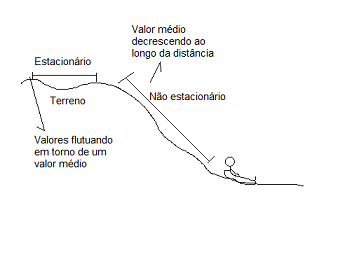
\includegraphics[width=0.8\textwidth,natwidth=610,natheight=642]{estc.png}	
\caption{Exemplo estacionaridade com um perfil topográfico. Região estacionária é plana, enquanto a região não-estacionária apresenta caimento constante.}
\label{estc}
\end{figure}

\section{Decomposição da função aleatória} \label{residuo}

Toda função aleatória $Z(x)$ pode ser dividida em dois componentes:  um valor de tendência e um de resíduo. Tal como uma combinação de variáveis aleatórias regionalizadas a função aleatória também é uma variável aleatória, possuindo um valor médio e uma distribuição de probabilidades para cada suporte x considerado. Como definido na seção anterior sob a hipótese de estacionaridade de segunda ordem temos um valor médio constante da função aleatória por todo o domínio. Denotaremos m como sendo o valor desta tendência (trend) da função aleatória. Retirado o valor médio desta função aleatória temos então o resíduo, dependente do suporte x considerado. Logo definimos que:

\begin{equation}\label{eq0:Decomposicaovariavel}
Z(x) = Y(x) + m(x)
\end{equation}

Em que $m(x)$ é o valor médio da função aleatória dependente da posição no espaço x e $Y(x)$ é o resíduo. Em muitos casos na mineração temos uma estrutura de controle no depósito mineral que cria condições de formação dado um viés ao longo do espaço. Uma falha na rocha ou um enriquecimento supergênico pode fazer com que determinado elemento se concentre ou disperse ao longo de uma direção. 

\section{Momentos estatísticos}


Momentos estatísticos são funções que caracterizam o comportamento de uma variável aleatória. Como estas assumem valores diferentes de acordo com sua probabilidade associada, podemos tentar definir seu valor mais provável, o grau de dispersão destes valores entre outros parâmetros. 

Duas propriedades mais comuns de uma variável aleatória são seus momentos de inércia de primeira e segunda ordem. Estes são definidos pelo valor esperado. A definição de valor esperado de uma variável aleatória pode ser representado pela equação \eqref{eq1:Valor_esperado} 

\begin{equation}\label{eq1:Valor_esperado}
E\left(Z\right)= \int_{-\infty}^{+\infty} p\left(z\right)zdz
\end{equation}

Onde z é uma realização da variável aleatória $p(z)$ é a sua probabilidade associada. Em outros termos a esperança matemática é nada mais que uma média ponderada da variável aleatória pela sua probabilidade, ou o valor mais provável de uma variável aleatória. Na geoestatística estamos interessados em estimar este parâmetro a partir de amostras, o que torna conveniente atribuir o valor esperado em sua forma discreta tal como demonstrado na equação \eqref{eq2:Valor_esperado_discreto}

\begin{equation}\label{eq2:Valor_esperado_discreto}
	E\left(Z\right)= \sum_{i=-\infty}^{+\infty}p\left(z_i\right)z_i
\end{equation}

A esperança matemática é um operador que apresenta uma série de propriedades que são normalmente utilizadas para demonstrar relações na geoestatística. Seja c uma constante real e Z uma variável aleatória, temos que:

\begin{equation}\label{eq3:Propesperancamatematica}
E\left(cZ\right)= cE\left(Z\right)
\end{equation}

No caso do valor médio de uma variável aleatória ser constante, temos que a esperança matemática de um valor médio é o próprio valor médio. Essa propriedade é interessante ser ressaltada nos casos em que consideraremos a hipótese de estacionaridade de segunda ordem: 

\begin{equation}\label{eq4:Propesperancamatematica2}
E\left( E(Z) \right)= E(c) = c
\end{equation}

O operador esperança matemática é comutativo, isso significa que:

\begin{equation}\label{eq5:Propesperancamatematica3}
E\left( Y +  Z\right)= E(Y) + E(Z)
\end{equation}


Não conhecemos o termo $p\left(z_i\right)$ da equação que corresponde à probabilidade de uma realização da variável z ocorrer em ponto, mas podemos inferí-la a partir de sua correlação com amostras na região. Na geoestatística linear o termo $p\left(z_i\right)$ se torna uma constante que é estimada a partir da correlação linear entre um ponto desconhecido e as amostras em seu entorno. Tal como descrito na equação \eqref{eq3:Media_ponderada}

\begin{equation}\label{eq3:Media_ponderada}
E\left(Z(x)\right)= \sum_{i=0}^{n}\lambda_iz(x_i)
\end{equation}

Onde i é o índice das amostras situadas ao arredor de um suporte x a ser estimado e $\lambda_i$ é o ponderador de cada estimativa . Os valores mais correlacionados com a distância e disposição das amostras contribuirão com uma maior probabilidade associada à média local.  

Da mesma forma podemos definir o momento estatístico de segunda ordem centrado, também chamado de variância, como \eqref{eq4:CapVariancia}:

\begin{equation}\label{eq4:CapVariancia}
Var\left(Z\right)= E\left( Z - E\left( Z\right) \right)^2
\end{equation} 

Por uma simples transformação podemos definir a variância de uma variável aleatória como descrito na prova abaixo:

\begin{proof} 	 
$Var\left( Z \right)= E\left( Z -E(Z) \right)^2$  \\
$Var\left(Z \right)= E\left( Z^2 -2ZE\left( Z\right)+ E(Z)^2 \right)$ \\
$Var\left(Z \right)= E(Z^2) -E(2ZE(Z)) +E(Z)^2$  \\
$Var\left(Z \right)= E(Z^2) -2E(Z)E(Z) +E(Z)^2$  \\
$Var\left(Z \right)= E(Z^2) -2E(Z)^2 +E(Z)^2$ \\
$Var\left(Z \right)= E(Z^2) - E(Z)^2$
\end{proof}

O momento estatístico mais importante para a geoestatística é a covariância, sendo definida como o grau de dependência entre duas variáveis distintas Z e Y, por exemplo. Definimos a relação segundo a equação \eqref{eq6:CapCorrelacao}: 

\begin{equation}\label{eq6:CapCorrelacao}
C\left(Z,Y\right)= E\left( (Z-E(Z)) (Y-E(Y)) \right)
\end{equation}

No caso em que as médias de Y e Z são iguais a covariância pode ser escrita como: 
\begin{proof}
$E(Z) = E(Y) = m $
\\$C\left(Z,Y\right)= E\left( (Z-m) (Y-m) \right)$
\\$C\left(Z,Y\right)= E\left( ZY - Zm - Ym +m^2 \right)$
\\$C\left(Z,Y\right)= E(ZY) - E(Zm) - E(Ym) +E(m^2) $
\\$C\left(Z,Y\right)= E(ZY) - mE(Z) - mE(Y) +E(m^2) $
\\$C\left(Z,Y\right)= E(ZY) - m^2 - m^2 +m^2$
\\$C\left(Z,Y\right)= E(ZY) - m^2$
\end{proof}

Essa demonstração é importante quando realizarmos as demonstrações da krigagem simples e ordinária posteriormente, utilizando a hipótese de estacionaridade de segunda ordem. A correlação e a variância são numericamente iguais quando consideradas as mesmas variáveis aleatórias. Se Y = Z podemos dizer que:

\begin{proof}
$ C\left(Z,Y\right) = E\left( (Z-E(Z)) (Y-E(Y)) \right) $
\\$C\left(Z,Z\right) = E\left( (Z-E(Z))(Z-E(Z)) \right)$
\\$C\left(Z,Z\right) = E\left( Z-E(Z) \right)^2$
\\$C\left(Z,Z\right) = Var(Z)$
\end{proof}

Todas essas demostrações realizadas em uma variável aleatória qualquer também são aplicáveis nos casos das variáveis aleatórias regionalizadas. 

\section{A função variograma e a função covariograma}

Como demonstrado na seção anterior podemos definir momentos estatísticos que representam características das variáveis aleatórias que definimos. Conceituamos a função covariância como sendo a esperança matemática do produto de duas variáveis aleatórias subtraído dos seus valores médios. Apesar de não estarmos interessados primordialmente na distribuição de probabilidades da nossa função aleatória é interessante definir o grau de correlação entre diversas variáveis aleatórias regionalizadas ao longo do nosso domínio. Definiremos agora a chamada função covariograma, que nada mais é que a correlação entre as variáveis aleatórias regionalizadas separadas de um vetor h.  

A função covariograma é então definida como sendo a covariância entre a função aleatória separada de um vetor h entre as variáveis aleatórias regionalizadas consideradas. Logo temos que : 

\begin{equation}\label{eq6:Covariograma}
C\left(h\right)= E\left( (Z(x)-m(x)) (Z(x+h)-m(x+h)) \right)
\end{equation}

 A função covariograma depende unica e exclusivamente do vetor considerado e não do suporte x das variáveis associadas. Em outros termos ela é dependente unicamente do fenômeno gerador do depósito e não da posição considerada para o seu cálculo. 

Sob a hipótese de estacionaridade de segunda ordem podemos transformar a função covariograma na seguinte relação:

\begin{proof}
$ m(x) = m\forall x \in D$
\\$ C\left(h\right)= E\left( (Z(x)-m) (Z(x+h)-m) \right)$
\\$ C\left(h\right)= E\left( (Z(x)Z(x+h)-Z(x)m-Z(x+h)m+m^2) \right)$
\\$C\left(h\right)= E(Z(x)Z(x+h))-m^2-m^2+m^2=E(Z(x)Z(x+h))-m^2$
\end{proof}

Outra função também importante a ser definida é o variograma. O variograma pode ser definido segundo a seguinte equação: 

\begin{equation}\label{eq6:Variograma}
2\gamma\left(h\right)= E\left( Z(x+h)-Z(x) \right)^2
\end{equation}

Sob a hipótese de estacionaridade de segunda ordem podemos transformar a função variograma na função covariograma  tal como demonstrado na relação a seguir.

Denotaremos agora a variância à priori do fenômeno como sendo a covariância para um vetor de tamanho zero C(0)=Cov(Z(x),Z(x))=$\sigma^2(0)$. 

Segundo a hipótese de estacionaridade de segunda ordem a variância de uma variável aleatória C(0)=c$\forall$ x $\in$ D:

\begin{proof}		
$ \gamma(h) = C(0) - C(h)$
\\$ E\left( Z(x+h)-Z(x) \right)^2/2 = C(0)-E(Z(x)Z(x+h))+m^2$\\
\\Devido a hipótese de estacionaridade de segunda ordem podemos decompor C(0) obtendo a seguinte relação:\\
$2C(0) = E(Z(x+h)^2)-m^2 + E(Z(x)^2)-m^2$\\
\\Isso nos leva à: \\
$ E\left( Z(x+h)-Z(x) \right)^2 = E(Z(x+h)^2)-m^2 + E(Z(x)^2)-m^2-2E(Z(x)Z(x+h))+2m^2$
\\$ E\left( Z(x+h)-Z(x) \right)^2 =E(Z(x+h)^2) + E(Z(x)^2)-2E(Z(x)Z(x+h))$
\\$ E\left( Z(x+h)-Z(x) \right)^2 =E(Z(x+h)^2 + Z(x)^2-2Z(x)Z(x+h))$
\\$ E\left( Z(x+h)-Z(x) \right)^2 =E\left( Z(x+h)-Z(x) \right)^2$
\end{proof}

No caso em que haja um valor de trend tal que a média seja dependente do suporte indicado (m(x)) a transformação da função covariância na função variograma pode ser realizada da mesma maneira, considerando que neste caso $m(x) \neq m(x+h)$. 

\section{Valor de variograma médio}

Como definido nas seções anteriores, o variograma é uma ferramenta estatística direcional, que depende exclusivamente do vetor associado e o fenômeno representado. Em alguns casos é interessante para nós definirmos um variograma médio, como sendo o valor da média dos variogramas dentro de um suporte determinado. Segundo a equação \eqref{eq7:Variogramamedio} definimos o variograma médio dentro de um suporte V contendo pontos nas posições x e y como abaixo:

\begin{equation}\label{eq7:Variogramamedio}
\bar{\gamma } (V) =\frac{1}{VV'} \int_{V(x)} \int_{V(x')} \gamma (Z(x)-Z(x'))dx dx'
\end{equation}

Em que x é um ponto no suporte V(x) e x' é um ponto no suporte V(x'). Na maioria das vezes a função integral não faz sentido no caso contínuo, já que calculamos o valor de $ \bar{\gamma }$ a partir de pontos discretos em volume. Neste caso definimos sua forma discreta segundo a equação \eqref{eq8:Variogramamedio} para nxn' pontos situados dentro de um volume determinado.  

\begin{equation}\label{eq8:Variogramamedio}
\bar{\gamma } (V) = \frac{1}{n n'}\sum_{i=1}^{n}\sum_{j=1}^{n'} \gamma (Z(x_{i})-Z(x_{j}))
\end{equation}

Estas equações serão importantes para definir questões de mudança de suporte nas estimativas. Em outras palavras, estimar em volumes e formas diferentes na geoestatística cria condições de variabilidade diversas. O valor médio de um painel de lavra subterrânea de algumas centenas de metros de extensão possui variabilidade totalmente diferente em relação à um bloco de um mina com algumas dezenas de metros apenas. 

\section{A variância de extensão}

Consideremos o exemplo demonstrado na figura \ref{estm}. Temos o ponto $Z(x_(0))$ que desconhecemos e queremos determinar sua estimativa a partir dos pontos de 1 a 4 determinados ao seu arredor. Poderíamos apenas tirar a média destes valores, mas isso não levaria em consideração a correlação espacial entre as amostras e sua posição no espaço. Seria interessante também encontrar uma estimativa que possuísse o menor erro possível. A variância de extensão é a medida que demonstra quanto do erro tomamos por estimar um ponto a partir de uma combinação linear de amostras. 

\begin{figure}
\centering
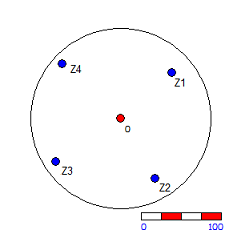
\includegraphics[width=0.8\textwidth,natwidth=610,natheight=642]{estm.png}	
\caption{Ponto $Z(x_{0})$ a ser estimado a partir de outros 4 pontos situados ao seu arredor}
\label{estm}
\end{figure}

Considere o sinal * como sendo um valor estimado de uma variável aleatória. No ponto 0 o erro de estimativa pode ser demonstrado segundo a equação \eqref{eq9:errestm}

\begin{equation}\label{eq9:errestm}
\varepsilon (Z^{*}(x_{0})) = Z^{*}(x_{0}) -Z(x_{0}) 
\end{equation}

Podemos estimar o valor esperado de $Z^{*}_{0}$ como sendo uma média ponderada dos valores amostrais de 1 a 4, logo temos que: 

\begin{equation}\label{eq9:errestm2}
\varepsilon (Z^{*}(x_{0}) = \sum_{i=1}^{4}\lambda _{i}Z(x_{i}) -Z(x_{0})   
\end{equation}

Para que o estimador não seja enviesado, devemos assumir que a esperança do erro de estimativa seja igual a zero. Considerando a hipótese de estacionaridade do valor médio, temos que: 

\begin{proof}
$E(\varepsilon (Z^{*}(x_{0}))) = E(\sum_{i=1}^{4}\lambda _{i}Z(x_{i}) -Z(x_{0})) = 0 $
\\$\sum_{i=1}^{4}\lambda _{i}E(Z(x_{i})) -E(Z(x_{0})) = 0 $
\\$\sum_{i=1}^{4}\lambda _{i}m -m = 0 $ 
\\$\sum_{i=1}^{4}\lambda _{i} = 1 $  	
\end{proof}


O mesmo pode ser provado para um valor de trend (m(x)). A variância do erro de estimativa pode ser então determinada segundo a prova abaixo. Além disso, consideramos que o somatório dos ponderadores $\sum_{i=1}^{4}\lambda _{i}=1$ :

\begin{proof}
$\sigma ^2\left (  \varepsilon (Z^{*}(x_{0})) \right )= E\left (\sum_{i=1}^{4}\lambda _{i}Z(x_{i}) -Z(x_{0}) \right )^2$
\\
$= E\left (\sum_{i=1}^{4}\sum_{j=1}^{4}\lambda _{i}\lambda _{j}Z(x_{i})Z(x_{j}) -\sum_{j=1}^{4}2\lambda _{i}Z(x_{i})Z(x_{0}) +Z(x_{0})^2 \right)$
\\
$= \sum_{i=1}^{4}\sum_{j=1}^{4}\lambda _{i}\lambda _{j}E(Z(x_{i})Z(x_{j})) -\sum_{i=1}^{4}2\lambda _{i}E(Z(x_{i})Z(x_{0})) +E(Z(x_{0})Z(x_{0}))$
\\ \\
Adicionando e retirando o valor da média m no problema temos:\\ \\
$= \sum_{i=1}^{4}\sum_{j=1}^{4}\lambda _{i}\lambda _{j}E(Z(x_{i})Z(x_{j}))-m^2 -\sum_{i=1}^{4}2\lambda _{i}E(Z(x_{i})Z(x_{0})) + 2m^2 +E(Z(x_{0})Z(x_{0})) -m^2$
\\
$= \sum_{i=1}^{4}\sum_{j=1}^{4}(\lambda _{i}\lambda _{j}E(Z(x_{i})Z(x_{j}))-m^2) -\sum_{i=1}^{4}2(\lambda _{i}E(Z(x_{i})Z(x_{0})) - m^2) +(E(Z(x_{0})Z(x_{0})) -m^2)$
\\
$= \sum_{i=1}^{4}\sum_{j=1}^{4}\lambda _{i}\lambda _{j}Cov(Z(x_{i}),Z(x_{j}))-\sum_{i=1}^{4}2\lambda _{i}Cov(Z(x_{i}),Z(x_{0}))+Cov(Z(x_{0}),Z(x_{0}))$

\end{proof}

O mesmo pode ser realizado considerando um valor de trend (m(x)). A variância do erro de estimativa, também chamada de variância de extensão, denotada como $\sigma^{2}_{e}$ é composta de três partes, uma com a autocovariância entre as amostras a serem utilizadas, a covariância entre o ponto estimado e as amostras e a variância do ponto estimado. 

\section{Krigagem}

O termo krigagem foi criado em homenagem a Daniel G. Krige que iniciou os trabalhos de geoestatística nas minas de ouro na África do Sul. Basicamente a krigagem nada mais é do que encontrar os valores dos ponderadores que minimizam a variância de estimativa, logo podemos definir a krigagem como sendo o conjunto de equações determinado por \eqref{eq11:krig}:

\begin{equation}\label{eq11:krig}
\frac{\partial }{\partial \lambda _{i}} \sigma ^{2}_{e}=0|\forall i  
\end{equation}

Utilizando a demonstração da seção anterior conseguimos verificar que o sistema de krigagem leva às seguintes equações. Para isso basta expandir a série para cada amostra considerada e derivar parcialmente cada um dos valores \eqref{eq11:krig_exp}: 

\begin{equation}\label{eq11:krig_exp}
\sum_{i=1}^{n}\lambda _{i}Cov(Z(x_{i}),Z(x_{j}))= Cov(Z(x_{i}),Z(x_{0}))|\forall j
\end{equation}

Diversos tipos de krigagem são determinadas a partir desta solução simples. Cada um dos sistemas possuí restrições quanto as hipóteses de cada modelo tornando o sistema de equações parciais em um problema de minimização com restrições, utilizando o operador lagrangiano, tal como demonstrado em \eqref{eq12:kriglamb}, sabemos que o gradiente do erro de estimativa deve ser ortogonal à restrição indicada. 

\begin{equation}\label{eq12:kriglamb}
\nabla \sigma ^{2}_{e}\bot \mu R' 
\end{equation}

Tal que R é uma restrição dada aos pesos no sistema de krigagem e $\mu$ é o operador lagrangiano. R' é portanto a derivada parcial da restrição em relação aos ponderadores. Essa restrição pode estar associada à uma condição de não viés do estimador ou de outra hipótese estabelecida.  


\section{A variância de dispersão}

Uma das maiores contribuições da geoestatística para a mineração e para efeitos de engenharia foi o conhecimento sobre a variabilidade em escala dos fenômenos espaciais. Na maioria das vezes estamos interessados em determinar o valor esperado de uma variável aleatória, sendo que esta pode apresentar uma dispersão, ou seja, o valor médio pode se situar dentro de limites desconhecidos. 

É bem intuitivo pensarmos que o valor médio estimado tende a depender do suporte considerado. Um volume muito grande de um painel de uma mina subterrânea estimado com seis ou sete furos de sondagem é bem mais preciso que o valor estimado de um bloco de minério de 10cm de comprimento.

A variância de dispersão é uma medida de quanto um volume a ser estimado pode variar segundo uma informação de um suporte diferente pode fornecer. Observe a figura \ref{var_disp}. No item A temos o valor médio das amostras contidas dentro do bloco como sendo uma estimativa daquele volume. A variância dos dados é tomada como sendo a variância das amostras A pelo valor médio dentro daquele suporte. A média de diversos blocos diferentes, como demonstrado em B relata a variância de dispersão. Neste caso temos uma medida qualitativa de quanto a informação de um suporte pode influenciar na estimativa de outro. 

\begin{figure}[H]
\centering
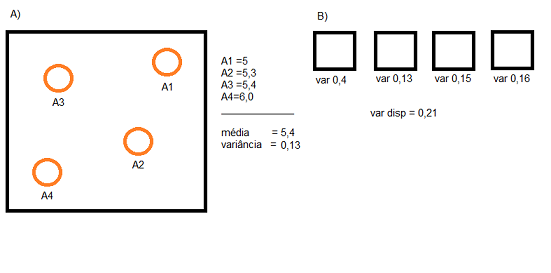
\includegraphics[width=0.8\textwidth,natwidth=610,natheight=642]{var_disp.png}
\caption{Exemplo para variância de dispersão A) Um bloco sendo estimado com valores de amostra laranja contido dentro dele b) Variância de dispersão como a média dos valores de variância para cada bloco}
\label{var_disp}
\end{figure}

Definimos a variância de dispersão de um suporte v dentro de um suporte V como definido na equação \eqref{eq8:Var_disp}

\begin{equation}\label{eq8:Var_disp}
D^{2}(V/v)=E[S^{2}(Z_{v}(x))]=E\left[\frac{1}{n}\sum_{i=1}^{n}\left(Z_{v}(x_{i})-Z_{V}(x)\right)^2\right]
\end{equation}


Note que $Z_{V}$ não necessariamente precisa ser a média de valores contidos dentro do suporte V.

Podemos utilizar qualquer estimativa para determinar o valor da variância de dispersão, podendo ser utilizada até mesmo o valor krigado, em que veremos em seções posteriores. A variância de dispersão é uma medida da entropia da informação e o quão ela influencia na estimativa em um dado suporte. 

\section{Exercícios}

\begin{enumerate}
	\item Enumere em uma lista todas as variáveis aleatórias regionalizadas que você possui em seu objeto de estudo. Indique ao lado se elas são somáticas ou não. Ex.: Teor-> somático, Condutibilidade hidráulica -> não somático.
	\item Cinco ações de uma mineradora possuem rentabilidade de 5, 10,20,4 e 5 Unidades monetárias. Se a probabilidade de renda destas ações forem iguais a 40\%, 35\%, 10\%, 10\% e 5\% qual é o valor esperado para a renda de todas as ações. Resp.:8.15 UM
	\item Cinco amostras possuem valor de teor iguais a 2\%, 2.5\%,2.3\%,2.1\% e 2.7\%. Se o volume das amostras é de 5,4,3,5 e 7 $cm^3$ qual é o teor médio das amostras. Resp.: 2,34\%
	\item Prove que o valor do resíduo da função aleatória é perpendicular à sua tendência, ou seja $Cov(R,m) = 0 \forall x \in D$ sendo D o valor do depósito.
	\item Prove que a covariância de duas variáveis aleatórias independentes seja igual a zero. Dica.: Tome o valor de $E(XY) = E(X)E(Y)$
	
\end{enumerate}

 